\chapter{\LaTeX: Making Beautiful Documents}\label{ch:latex}
40 pages

\section{Why \LaTeX?}
Most people need to write text documents from time to time, be it a CV, an article or a school assignment. Especially if you're writing something you'll use in your profession, you likely want it to \emph{look} professional which usually is not the case when you use tools like Microsoft Word or LibreOffice Writer. With these what-you-see-is-what-you-get (WYSIWYG) tools, the author spends time manually tweaking how stuff looks; where the title is, which fonts to use, text sizes, and placement. Most of us are not interested enough in typography to do this right. In comparison, using \LaTeX{}, the writer focuses on what stuff \emph{is}, rather than how stuff \emph{looks}. By telling \LaTeX{} ``this is a title'', or ``this is a new paragraph'' \LaTeX{} itself will figure out the proper formatting. It may seem unfamiliar at first that \LaTeX{} decides how stuff looks, indeed many novices try to force \LaTeX{} to display stuff in a particular way. My advice: don't!

\LaTeX{} certainly comes with a higher learning barrier before you can use it than WYSIWYG tools, but once you get familiar with it, I think you'll find that using it actually isn't that much slower, and it produces much better results. You may find a shift in what you spend time on: less time manually placing stuff, more time looking for how to do ``this thing'' with \LaTeX{} on the internet.

Other professional typesetting tools exist as well, but \LaTeX{} is very well developed and by far the most widespread, at least in scientific publications and books. We'll also see how to use it for making slideshow presentations, thus replacing tools such as Microsoft PowerPoint. If there's one typesetting tool you want in your toolbox to it's definitely \LaTeX{}.

\section{Which tools you need}
\LaTeX{} can be written in any plain text editor (like Notepad if you're using Windows) and stored to a file ending with .tex. The .tex file is then \emph{compiled} to generate a .pdf-file using the command line tool \verb|pdflatex|. However, most users prefer a more specialized text editor which runs \verb|pdflatex| for you. Most such editors also supports highlighting, i.e.\ the application of different colors to different parts of the code to make it more readable. Many good editors exist, but we will use Texmaker which works on both Linux, OS X and Windows.

To get \LaTeX{}, you need to install a \LaTeX{}-distribution on your computer. There are several of them, but the code you write is the same for all of them. Proceed according to your operating system to install a \LaTeX-distribution and Texmaker.

\subsection{Linux}
On Linux, TeX Live is the recommended distribution. On Ubuntu, Mint or Debian Linux, you can install TeX Live and Texmaker using the following command:
\begin{verbatim}
$ sudo apt-get install texlive-full texmaker
\end{verbatim}

\subsection{OS X}
For OS X, MacTeX is the recommended distribution. It is the essentially the same as TeX Live but adds some compatibility to OS X. Download and install MacTeX and Texmaker from the following links:

\begin{verbatim}
http://tug.org/mactex
http://www.xm1math.net/texmaker
\end{verbatim}

\subsection{Windows}
For Windows either TeX Live or MiKTeX can be used, but many find MiKTeX slightly easier to handle. Install MiKTeX and Texmaker from the following links:

\begin{verbatim}
http://www.miktex.org
http://www.xm1math.net/texmaker
\end{verbatim}

\section{Our first document}

\subsection{A minimal example}
We will start by going through \reflst{latex:minimal} which is about the minimum code required to start a new document. The left part is the source code while the right part demonstrates the output produced by the code. The actual result will necessarily be slightly different, since it will be placed in its own document with its own page and formatting, but a demonstration may be instructive in some of the examples nevertheless.

\begin{listing}
	\rule{\textwidth}{0.4pt}
	\begin{minipage}[t]{0.49\textwidth}
		\inputminted[frame=none]{latex}{latex/first.tex}
	\end{minipage}\hfill\vline\hfill
	\begin{minipage}[t]{0.49\textwidth}
		Here is some text.
	\end{minipage}\\[0.5em]
	\rule{\textwidth}{0.4pt}
	\caption{A (near-)minimal \LaTeX{} document}
	\label{lst:latex:minimal}
\end{listing}

Notice that all \LaTeX{}-\emph{commands} start with a backslash, and may be followed by mandatory \emph{arguments} in curly braces, and optional arguments (\emph{options}) in square brackets like this:

\latexone|\command[option1,option2]{argument1}{argument2}|
\noindent Such ``rules'' for how commands are structured is usually referred to as \emph{syntax}.

\subsubsection{Document class}
The first command in any document is \latexin{\documentclass} which tells \LaTeX{} what kind of document it is. Some possible arguments are shown in \reftab{latex:documentclass}. The option \latexin{a4paper} tells \LaTeX{} to produce a document in paper size A4.

\begin{table}
	\centering
	\caption{Document classes}
	\begin{tabular}{ll}
	\hline
	\latexin{book}		&	For books. Asymmetric margins, smaller margin towards						\\
						&	the cover of the book.													\\
	\latexin{report}		&	For reports and somewhat big documents.									\\
	\latexin{article}	&	For articles and smaller documents. Excludes chapters.					\\
	\latexin{beamer}		&	For	slideshow presentations using the Beamer package.						\\
	\latexin{curve}		&	For CVs using the Curve package.
	\end{tabular}
	\label{tab:latex:documentclass}
\end{table}

Some people think \LaTeX{} produces wastefully large margins, and tries to force it to use smaller margins. However, typographists know that the mind gradually gets unfocused by the end of the line, and refocuses again for the next line. Henceforth, \LaTeX{} takes care of not making lines too long. Books are often written in the slightly smaller format B5 to reduce wasted paper, while magazines and scientific journals often split the pages in two columns using the option \latexin{twocolumn}, e.g.:

\latexone|\usepackage[a4paper,twocolumn]{article}|
\noindent Consider this if it is important for you to reduce wasted space.

\latexin{\documentclass} also support options for other paper sizes, font sizes, etc.\ which you can find on the internet whenever you need it.

\subsubsection{Packages}
Next, the functionality of \LaTeX{} can be expanded by including \emph{packages} which provides more features (similar to \emph{modules} in Python or \emph{libraries} in other languages). This is done by the \mintinline{latex}{\usepackage} command, one per package you want to use. To begin with, we need three packages: \latexin{inputenc} specifies the \emph{character encoding} which is used in the .tex files. We'll get back to this. \mintinline{latex}{fontenc} determines the \emph{font encoding} to be used in the .pdf-file. We won't dig into this but it should usually be T1. Finally, \mintinline{latex}{babel} specifies the written language.

The next new thing we'll encounter is an \emph{environment}. An environment starts with a \latexin{\begin} and ends with an \latexin{\end}, and affects anything in between. The \latexin{document} environment is where you write what actually goes into the document. Everything before it, is called the \emph{preamble} and is not actually printed to the document. Here we only have the text ``Here is some text.'' and a \emph{comment}, which is text \LaTeX{} completely ignores. Everything following a \% is a comment. Comments are only for your own convenience; you may write comments for instance about what commands does, why you chose to write something the way you did, etc.

\subsection{Character Encoding}
Whenever text is stored in a file it is represented by strings of zeros and ones (\emph{binary digits} or just \emph{bits}) according to a \emph{character encoding standard}. An early standard is the \emph{ASCII} standard (American Standard Code for Information Interchange) which uses 7 bits to represent letters. For instance, ``A'' is represented by the binary number 1000001 which maps to 65 when converted to the decimal system. Since 7 bits can only encode 128 characters, only the most common characters were included in the ASCII standard. By expanding it with one bit, 128 characters more could be encoded. However, this is still not enough for all kinds of languages, and as a result, different 8 bit encodings exist depending on where you're from. One of the most popular is ISO-8859-1 which includes the letters used in Western European languages. However, then you cannot use letters outside of this standard. UTF-8, on the other hand, is a very clever encoding which circumvents this problem by using 8 bits (or one byte) for the most common characters but may use up to four bytes for rarer characters. As such, UTF-8 has a wide range of characters and should cover all your needs while not making the text documents much larger. I recommended storing all .tex files as UTF-8 to avoid encoding problems.

In Texmaker you can ensure files are stored as UTF-8 by going to Options$\rightarrow$ Configure Texmaker (see \reffig{latex:texmaker}), open the ``Editor'' pane and make sure ``Editor Font Encoding'' is set to UTF-8. Finally, the \LaTeX{} compiler needs to know the encoding to decode it correctly as well. This is what we've told it in the option for the \latexin{inputenc} package in \reflst{latex:minimal}. A common pitfall is that the \latexin{inputenc} option does not match the actual encoding used in the file which causes local/special (non-ASCII) characters to look like other symbols.

\begin{figure}
	\centering
	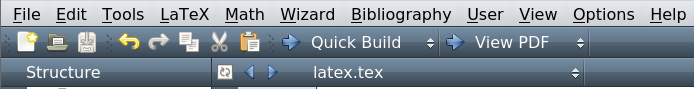
\includegraphics[width=\textwidth]{graphics/texmaker.png}
	\caption{Texmaker toolbar}
	\label{fig:latex:texmaker}
\end{figure}

\subsection{Compiling}
The next step is to compile our minimal example to turn it into a .pdf file. The minimal example from \reflst{latex:minimal} can be saved to a UTF-8 encoded file \texttt{main.tex} in a new folder. You \emph{do} want to create a separate folder for each document you write since \LaTeX{} generates lots of other files in this folder upon compilation.

One should be aware that people use different compilation strategies. Some people use the program \texttt{latex} which generates a .dvi file and then converts it to .pdf using a conversion tool, while we will use the program \texttt{pdflatex} which directly generates the .pdf file. Both of these are command line programs but Texmaker can run these commands so we don't have to. However, to better grasp what's going on behind the curtains, we will see how it's done both from the command line and from Texmaker. If you haven't read \refch{bash} yet, don't worry. You don't need to be able to run the commands to proceed this chapter.

\subsubsection{Using the command line}
To compile \texttt{main.tex} using the (Linux, OS X or Windows) command line, navigate to the folder where the file is, and simply run:
\begin{verbatim}
$ pdflatex main.tex
\end{verbatim}
and a file named \verb|main.pdf| will be created. If you got no errors you're done.

But computers are very literal and errors is the most common thing. If there's a typo somewhere in your code, e.g. a capital letter instead of a small one in a command, the document simply will not compile, but returns an error. The error messages may look cryptic at first, but they do tell what the error is and which line it is on. You can exit the failed compilation in the command line by typing ``x''. Try to sort out one error at a time, starting with the top one.

Sometimes, when you have an error in your code, and you can't figure out what it is, it may be useful to \emph{comment out} a block of lines. Texmaker supports commenting out multiple lines by marking them and hitting Ctrl+T. Uncommenting the marked lines is done by Ctrl+U. Another advice: Compile your document often to avoid a bunch of errors to accumulate. Fixing errors is perhaps the largest barrier when starting to program, but it gets a lot easier with a little experience.

\subsubsection{Using Texmaker}
Next: compile using Texmaker. We can use the arrow next to the ``Quick Build'' drop down menu (see \reffig{latex:texmaker}) to run any of the programs available from the drop down menu. As an example, we can choose ``PDFLaTeX'' and click the arrow, and to view it, we can click the arrow next to ``View PDF''. The ``Quick Build'' option is useful, since it can be configured to run a series of commands in sequence. If you again go to Options$\rightarrow$Configure Texmaker and select the ``Quick Build'' pane you can set Quick Build to ``PdfLaTeX + View PDF''. In the ``Commands'' pane, you can see exactly which commands Texmaker uses when running this programs. These are fine as they are. Now, when you choose ``Quick Build'' and click the arrow, the document will be compiled and displayed. Like when using the command line errors must be resolved to make the document compile.

You are advised to successfully compile \reflst{latex:minimal} before proceeding, and to experiment with the examples throughout the chapter as you go.

\section{Document Structure}
When we're writing a document, we likely want to structure it by splitting it into chapters. Chapters can again be split into sections, which again can be split into subsections and further on to subsubsections. The corresponding commands are, intuitively, \latexin{\chapter}, \latexin{\section}, \latexin{\subsection} and \latexin{\subsubsection}. You can see how these are used in \reflst{latex:structure} to structure the document. Numbering of chapters, sections and so on happen automatically.

\begin{listing}
	\inputminted{latex}{latex/structure.tex}
	\caption{A \LaTeX{} document with some structure and text}
	\label{lst:latex:structure}
\end{listing}

A chapter is a rather big, voluminous entity. The chapter title may well consume approximately half a page, like in this book. In smaller documents like articles, school assignments, etc., which may only be a few pages, this is not appropriate. The  \latexin{article} document class is suitable in such cases since it does not have chapters. There, sections are the highest structural level.

Further on, \LaTeX{} do not care if you write a whole paragraph in one line, or split it up into more lines. It will not break the lines where you do, but where it deems appropriate. To start a \emph{new} paragraph, you hit enter twice leaving a line open (line 14 in \reflst{latex:structure}). In \LaTeX{} documents text is not left-aligned but justified, i.e.\ spaces are stretched so that all lines end at the same point. New paragraphs are indicated by an indentation which is clearly visible among the justified lines.

In \reflst{latex:structure} we have also used the command \latexin{\lipsum[1-3]}. This is a command which fills the document with paragraphs one to three of some rather arbitrary sample text known as Lorem ipsum. Lorem ipsum is a piece of scrambled Latin text which is commonly inserted into a document or web page before you have any actual contents just to get a feel for how it will look. Repeating short fragments such as ``text text text'' produces patterns in the document which looks unnatural. \latexin{\lipsum}, however, is not provided by \LaTeX{} as-is but is rather provided to us by a package \latexin{lipsum}. To use \latexin{\lipsum}, we need to include this package in the preamble of our document (line 5 in \reflst{latex:structure}). The \LaTeX{}-distributions comes pre-loaded with a bunch of packages (especially TeX Live) so you will likely have most of them. If not, you'll need to install it separately.

As a side remark, you may notice the \latexin{\lipsum[1-3]} command in \reflst{latex:structure}. This command outputs paragraphs one to three of a text known as Lorem ipsum. Lorem ipsum is based on an old Latin text by Cicero, but scrambled to become senseless, and is typically used as dummy text in web pages and documents to see how it looks with contents. The disadvantage of just repeating for instance ``text text text ...'' over and over again is that it creates unnatural patterns in the text.

In \reflst{latex:structure} we have also used the command \latexin{\lipsum}. This is a command which fills the document by some rather arbitrary sample text at this spot known as Lorem ipsum. Lorem ipsum is a piece of gibberish latin text which is commonly inserted into a document or web page before you have any actual contents just to get a feel for how it will look. \latexin{\lipsum}, however, is not provided by \LaTeX{} as-is but is rather provided to us by a package \latexin{lipsum}. To use \latexin{\lipsum}, we need to include this package in the preamble of our document (line 5 in \reflst{latex:structure}). The \LaTeX{}-distributions comes pre-loaded with a bunch of packages (especially TeX Live) so you will likely have most of them. If not, you'll need to install it separately.

\subsection{Table of contents}
Since \LaTeX{} knows what are structural elements like chapters, sections, and so on, it can also auto-generate a table of contents for you. This is done with the \latexin{\tableofcontents} command on line 9. When compiling the document the first time, \LaTeX{} makes a list of all the structural elements and stores it in one of its auxiliary files. This list will be used when making the table of contents, but unfortunately will not be available until the next time you compile the document. Therefore, the first time you compile the document, the compiler will not be able to generate the table of contents properly. Likewise, if you do any changes in the structure of the documents, you will have to compile twice for table of contents to reflect those changes.

\subsection{Title page}
\LaTeX{} is able to auto-generate a simple title page for you using the command \latexin{\maketitle}. To do that, it needs to know the title of the document, the author, and/or the date of publication.

The commands \latexin{\title}, \latexin{\author} and \latexin{\date} can be put in the preamble to tell \LaTeX{} the title and author of the document, along with the date it was written/published.

 Here we have only a title page which is auto-generated by the \latexin{\maketitle} command, and the text ``Here is some text.''. Normal text can simply be written as-is and requires no special commands.


\subsection{Formatting}
Basically, \LaTeX{} takes care of formatting, but sometimes you may want to tell \LaTeX{} to emphasize a word. This is done using \latexin{\emph}. You generally do not tell \LaTeX{} to display text as bold, italic or underlined like in WYSIWYG programs, but rather to emphasize it. Then it is up to \LaTeX{} to emphasize it in the proper way (which normally is italic).

Comments are written using two backticks in the beginning of the quote, and two single quote marks at the end like this:

\latexone{``This is a quote''}

The reason for not just using a normal double quote mark is that various languages have different conventions of how quotation marks looks like, e.g. <<quote>>, ,,quote'' or "quote". When using two backticks and two single-quote marks, \LaTeX{} replaces them by the proper quotation marks for your language.

What do you think the command \latexin{\LaTeX{}} on line 18 in \reflst{latex:structure} do?

In \reflst{latex:structure} we have also used the command \latexin{\lipsum}. This is a command which fills the document by some rather arbitrary sample text at this spot known as Lorem ipsum. Lorem ipsum is a piece of gibberish latin text which is commonly inserted into a document or web page before you have any actual contents just to get a feel for how it will look. \latexin{\lipsum}, however, is not provided by \LaTeX{} as-is but is rather provided to us by a package \latexin{lipsum}. To use \latexin{\lipsum}, we need to include this package in the preamble of our document (line 5 in \reflst{latex:structure}). The \LaTeX{}-distributions comes pre-loaded with a bunch of packages (especially TeX Live) so you will likely have most of them. If not, you'll need to install it separately.

Make sure you understand each line in \reflst{latex:structure}. 

\subsection{Reserved characters}
While you can write text as normal in \LaTeX{}, some symbols are reserved for special use. For instance, if you write a \% (comment symbol), \LaTeX{} ignores everything else on that line. But what if you actually want to write \%? You can write reserved symbols by \emph{escaping} them with a backslash like this:

\latexone{We offer you an interest rate of 5\% }
The following characters are reserved for special use in \LaTeX{}:
\begin{verbatim}
# $ % ^ & _ { } ~
\end{verbatim} 

But they can be written as follows:

\latexone{\# \$ \% \^{} \& \_ \{ \} \~{} \textbackslash{}}


\subsection{Assignments}
To familiarize yourself a bit with \LaTeX{}, here's some small suggested assignments:
\begin{enumerate}
	\item Compile the document in \reflst{latex:structure} if you have not done so already.
	\item Experiment with changing the content. Try out some reserved characters.
	\item Change the language of the document to your native tongue. Use the internet to find the right option of the \latexin{babel} package. Hint: When you change the language of the babel package of an already existing document you need to delete the file \verb|main.aux| before compiling. This is because \verb|main.aux|, which is an auxiliary file \LaTeX{} uses, remembers the previously used language and this causes a conflict in the compiler. Not understanding why changing language fails is a common source of frustration.
	\item Change the document class to \latexin{article}. Unlike \latexin{book} and \latexin{report}, \latexin{article} does not spend almost half a page writing ``Chapter 1 - Introduction'', so for smaller documents (e.g.\ school assignments), \latexin{article} is a good document class to choose. \latexin{article} do not have chapters, so replace all chapters by sections, sections by subsections and subsections by subsubsections.
	\item Let's say we don't want to enumerate the subsubsections. Then you can replace \latexin{\subsection{something}} by \latexin{\subsection*{something}}
\end{enumerate}

\subsection{Splitting documents into several files}
As your project gets bigger, your \verb|main.tex| file may start looking like a mess and you just can't find the parts your looking for. In such cases, it is very useful to split the document into multiple files, for instance one file per chapter, section or any other appropriately sized chunks of text. The main file may then look like in \reflst{latex:multifiles}.

\begin{listing}
	\inputminted{latex}{latex/multifiles.tex}
	\caption{A .tex file with chapters in separate subfiles}
	\label{lst:latex:multifiles}
\end{listing}

The \latexin{\input} commands are replaced by the contents of the files specified as its argument. If the argument is \latexin{{introduction.tex}} or just simply \latexin{{introduction}} it searches for a file \verb|introduction.tex| in the same folder as \verb|main.tex|. You can also specify subfolders, like \latexin{{subfolder/introduction.tex}}, but I normally prefer to keep all .tex files in the same folder.

The introduction.tex file is demonstrated in \reflst{latex:introduction} and the conclusion.tex files is made in a similar manner.

\begin{listing}
	\inputminted{latex}{latex/introduction.tex}
	\caption{A chapter put into a separate file}
	\label{lst:latex:introduction}
\end{listing}

\section{References}

\section{Formatting}
Special characters, symbols, emphasize and quotes

\section{Lists}
itemize, enumerate

\section{Figures}
png vs. pdf, references, captions, inkscape

\section{Tables}

\section{Bibliography}

\section{New commands}

\section{Writing an Application}

\section{Writing a CV using CurVe}

\section{Writing a presentation using Beamer}